\documentclass[12pt]{article}
\usepackage[spanish]{babel}
\usepackage[utf8]{inputenc}
\usepackage[T1]{fontenc}
\usepackage{geometry}
\usepackage{graphicx}
\usepackage{hyperref}
\usepackage{enumitem}
\usepackage{float}
\usepackage{caption}
\usepackage{array}
\usepackage{longtable}

\geometry{margin=2.25cm}
\hypersetup{colorlinks=true,linkcolor=black,urlcolor=black}
\setlist[itemize]{leftmargin=*,itemsep=0.2em}
\setlist[enumerate]{leftmargin=*,itemsep=0.25em}
\captionsetup{font=small,labelfont=bf}

\newcommand{\boton}[1]{\textbf{#1}}
\newcommand{\menu}[1]{\textbf{#1}}
\newcommand{\campo}[1]{\textbf{#1}}
\newcommand{\estado}[1]{\texttt{#1}}

\title{Manual de usuario detallado\\Asociación Gent Gran de Castelldefels -- Gestión}
\author{}
\date{\today}

\begin{document}
\maketitle
\tableofcontents
\newpage

\section{Objetivo del manual}
Este manual explica de forma detallada el uso de GentGranBD, la aplicación de escritorio para la gestión de la Asociación Gent Gran de Castelldefels. Está dirigido a personal administrativo, coordinación de actividades y usuarios con permisos de administración.

El documento cubre:
\begin{itemize}
  \item Acceso a la aplicación y gestión de perfiles de conexión.
  \item Creación y mantenimiento de cursos académicos y trimestres.
  \item Alta, consulta, modificación, baja y documentación de socios.
  \item Inscripciones, reservas, pagos y participantes de cursos y viajes.
  \item Control de asistencia por actividad y trimestre.
  \item Gestión de LOPD y firma digital desde tablet o móvil.
  \item Gestión de profesores, voluntarios y usuarios de la aplicación.
  \item Importación desde Excel o CSV, copias de seguridad, restauraciones y actualizaciones.
\end{itemize}

Los nombres de menús, botones y campos se mantienen tal como aparecen en pantalla, normalmente en catalán. Cuando este manual indique ``pulse'', se refiere a hacer clic con el ratón o activar el control correspondiente.

\section{Conceptos básicos de trabajo}
\subsection{Estructura de la información}
La aplicación organiza los datos en varias áreas relacionadas:
\begin{itemize}
  \item \textbf{Socios}: personas dadas de alta en la entidad. Pueden tener datos personales, contacto, foto, fecha de alta, baja, observaciones, inscripciones, pagos, asistencia y documento LOPD.
  \item \textbf{Cursos académicos}: periodos de trabajo, normalmente anuales. Cada curso contiene cuatro trimestres.
  \item \textbf{Actividades}: cursos o viajes vinculados a un curso académico. Tienen responsable, precio, número máximo de plazas, descripción e inscritos.
  \item \textbf{Inscripciones}: relación entre un socio y una actividad. Pueden estar en estado \estado{INSCRIT} o \estado{RESERVA}.
  \item \textbf{Pagos}: importes asociados a una inscripción. Pueden estar en estado \estado{PENDENT}, \estado{PAGAT} o, cuando se editen desde la tabla, \estado{ANULAT}.
  \item \textbf{Clases y asistencia}: sesiones concretas de una actividad y marcas de presencia de cada participante.
  \item \textbf{Personal}: profesores y voluntarios que pueden figurar como responsables de actividades.
  \item \textbf{Usuarios}: cuentas que permiten entrar en la aplicación.
\end{itemize}

\subsection{Orden recomendado de uso inicial}
Para empezar a trabajar con una base nueva, siga este orden:
\begin{enumerate}
  \item Entre con un usuario administrador.
  \item Cree el curso académico vigente desde \menu{Arxiu > Gestionar Curs Acadèmic}.
  \item Revise las fechas de los cuatro trimestres.
  \item Cree profesores y voluntarios desde la pestaña \menu{Personal}.
  \item Cree cursos o viajes desde la pestaña \menu{Activitats}.
  \item Dé de alta socios o impórtelos desde Excel/CSV.
  \item Inscriba socios en actividades.
  \item Registre pagos y asistencia según avance el curso.
  \item Genere documentos e informes cuando sea necesario.
\end{enumerate}

\subsection{Convenciones visuales}
La interfaz utiliza patrones repetidos:
\begin{itemize}
  \item Los botones verdes suelen crear, añadir o confirmar.
  \item Los botones rojos eliminan o ejecutan acciones irreversibles.
  \item Los botones claros o secundarios abren opciones auxiliares, exportaciones o descartes.
  \item Las tablas muestran una fila por registro y se actualizan al buscar, guardar o eliminar.
  \item Los paneles de detalle muestran el registro seleccionado.
  \item Las fechas se muestran con formato día/mes/año o día-mes-año, según la ventana.
\end{itemize}

\section{Acceso a la aplicación}
\subsection{Pantalla de inicio de sesión}
Al abrir GentGranBD aparece la ventana \menu{Accés a Gent Gran}. En ella se selecciona la conexión a la base de datos y se introducen las credenciales de usuario.

\begin{figure}[H]
  \centering
  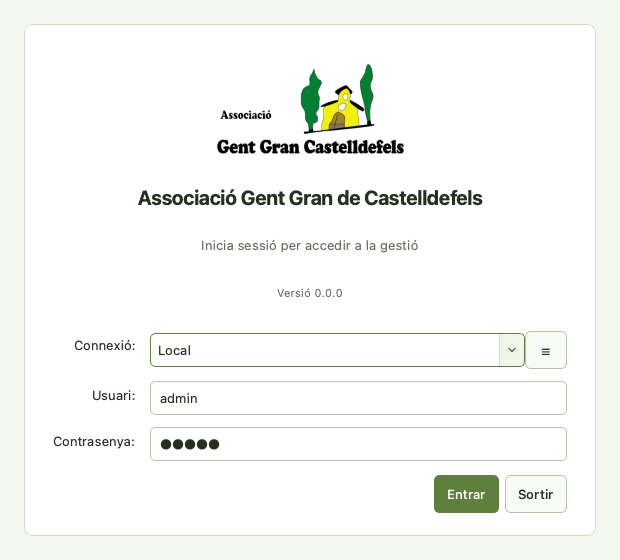
\includegraphics[width=0.70\textwidth]{./images/0_acces.png}
  \caption{Pantalla de acceso a la aplicación.}
  \label{fig:acceso}
\end{figure}

Campos y controles:
\begin{itemize}
  \item \campo{Connexió}: perfil de base de datos. Para un uso normal local, seleccione \menu{Local}.
  \item Botón de perfiles de conexión: abre la gestión de conexiones si se trabaja con bases externas.
  \item \campo{Usuari}: nombre del usuario de la aplicación.
  \item \campo{Contrasenya}: contraseña asociada al usuario.
  \item \boton{Entrar}: valida la conexión y las credenciales.
  \item \boton{Sortir}: cierra la ventana de acceso sin entrar.
\end{itemize}

\subsection{Perfiles de conexión}
El perfil \menu{Local} usa una base SQLite en el ordenador. También pueden configurarse perfiles PostgreSQL si la entidad trabaja con una base centralizada.

En un perfil externo se suelen indicar:
\begin{itemize}
  \item Nombre descriptivo del perfil.
  \item Host o servidor.
  \item Puerto.
  \item Nombre de base de datos.
  \item Usuario y contraseña de base de datos.
  \item Modo SSL.
\end{itemize}

Recomendación: si no sabe qué perfil usar, mantenga \menu{Local} o consulte con la persona responsable de la instalación.

\subsection{Errores habituales al entrar}
\begin{itemize}
  \item \textbf{Usuario o contraseña incorrectos}: revise mayúsculas, minúsculas y espacios.
  \item \textbf{Error de conexión}: el perfil seleccionado no es accesible o la base externa no responde.
  \item \textbf{Base nueva sin usuarios}: la aplicación puede crear el usuario inicial si no hay usuarios registrados.
  \item \textbf{Usuario desactivado}: contacte con un administrador.
\end{itemize}

\section{Ventana principal}
\subsection{Distribución general}
Después de iniciar sesión se abre la ventana principal. La barra superior contiene los menús \menu{Arxiu}, \menu{Ajuda} y, si el usuario es administrador, \menu{Administració}. Debajo aparecen las pestañas principales.

\begin{figure}[H]
  \centering
  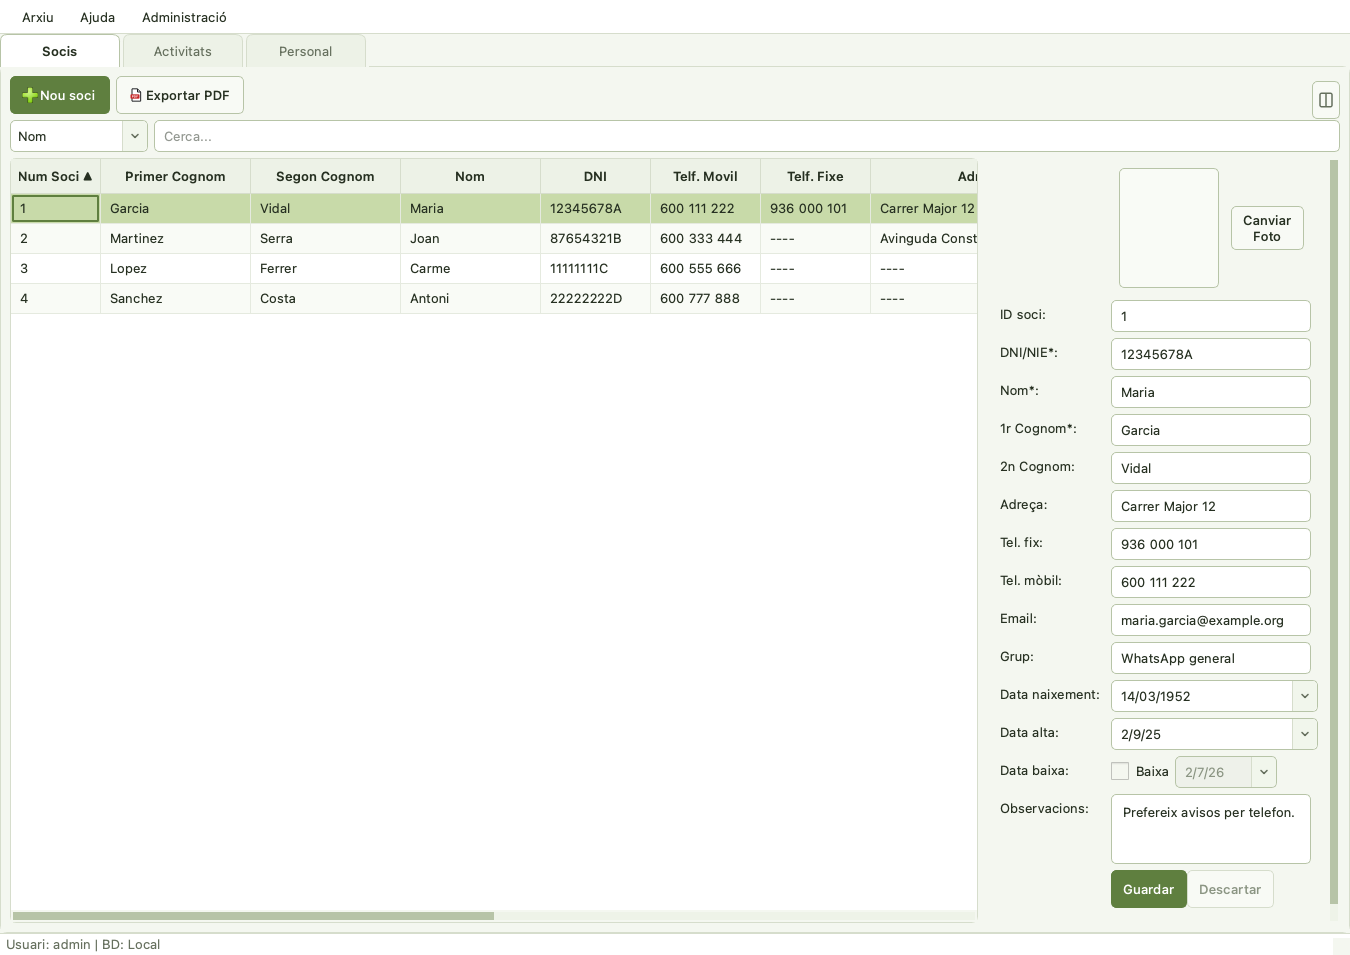
\includegraphics[width=\textwidth]{./images/1_principal.png}
  \caption{Ventana principal en la pestaña Socis.}
  \label{fig:principal}
\end{figure}

Pestañas:
\begin{itemize}
  \item \menu{Socis}: alta, consulta, modificación, baja, búsqueda y documentación de socios.
  \item \menu{Activitats}: gestión de cursos, viajes, participantes e informes.
  \item \menu{Personal}: profesores y voluntarios.
\end{itemize}

\subsection{Menú Arxiu}
El menú \menu{Arxiu} agrupa acciones generales:
\begin{itemize}
  \item \menu{Gestionar Curs Acadèmic}: abre la ventana de cursos académicos y trimestres.
  \item \menu{Importar Socis (CSV/Excel)}: carga socios desde un archivo de hoja de cálculo.
  \item \menu{Còpia de seguretat de la BD}: crea una copia de la base local. Solo para administradores.
  \item \menu{Restaurar BD des d'una còpia}: restaura una base local desde un archivo. Solo para administradores.
  \item \menu{Canviar contrasenya}: permite cambiar la contraseña del usuario actual.
  \item \menu{Tancar sessió}: cierra la sesión y vuelve a la pantalla de acceso.
\end{itemize}

\subsection{Menú Ajuda}
El menú \menu{Ajuda} permite:
\begin{itemize}
  \item \menu{Comprovar actualitzacions manualment}: busca nuevas versiones cuando se usa la aplicación empaquetada.
  \item \menu{Informació de la versió}: muestra versión de GentGranBD, modo de ejecución, versión de Python y ruta del ejecutable.
\end{itemize}

\subsection{Menú Administració}
Disponible únicamente para usuarios con rol \estado{ADMIN}. Incluye:
\begin{itemize}
  \item \menu{Usuaris}: creación, modificación, desactivación, eliminación y auditoría de usuarios.
\end{itemize}

\subsection{Barra de estado}
La barra inferior muestra el usuario activo y la conexión de base de datos. Es útil para confirmar si se está trabajando en la base local o en una base externa.

\subsection{Cambios pendientes}
Algunas pantallas tienen edición directa. Si cambia de pestaña, cierra sesión o instala una actualización con datos sin guardar, la aplicación puede pedir confirmación para guardar, descartar o cancelar la acción.

\section{Cursos académicos y trimestres}
\subsection{Finalidad}
El curso académico es imprescindible para organizar actividades. Una actividad siempre se vincula a un curso, y la asistencia se divide por trimestres. Si no existe un curso vigente, algunas acciones quedarán vacías o deshabilitadas.

\begin{figure}[H]
  \centering
  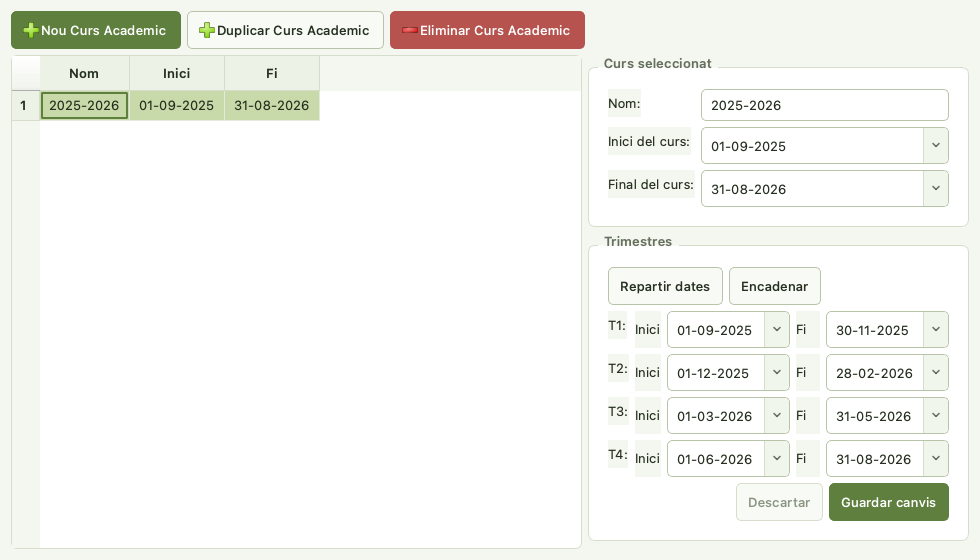
\includegraphics[width=0.92\textwidth]{./images/2_cursosAcademics.png}
  \caption{Gestión de cursos académicos y trimestres.}
  \label{fig:cursos}
\end{figure}

\subsection{Crear un curso académico}
\begin{enumerate}
  \item Abra \menu{Arxiu > Gestionar Curs Acadèmic}.
  \item Pulse \boton{Nou Curs Academic}.
  \item Revise el \campo{Nom del curs}. La aplicación propone un nombre basado en los años de inicio y fin.
  \item Indique \campo{Inici} y \campo{Fi}.
  \item Pulse \boton{Crear curs}.
  \item Compruebe que el nuevo curso aparece en la tabla.
\end{enumerate}

Al crear un curso se generan automáticamente los cuatro trimestres. Revise sus fechas antes de crear actividades.

\subsection{Editar fechas de curso y trimestres}
\begin{enumerate}
  \item Seleccione el curso en la tabla izquierda.
  \item Modifique \campo{Nom}, \campo{Inici del curs} o \campo{Final del curs}.
  \item En el bloque \menu{Trimestres}, ajuste las fechas de \campo{T1}, \campo{T2}, \campo{T3} y \campo{T4}.
  \item Pulse \boton{Guardar canvis}.
\end{enumerate}

Use \boton{Descartar} para abandonar los cambios no guardados y volver a los valores anteriores.

\subsection{Repartir fechas y encadenar trimestres}
\begin{itemize}
  \item \boton{Repartir dates}: divide automáticamente el rango del curso en cuatro periodos consecutivos.
  \item \boton{Encadenar}: conserva las fechas de fin y ajusta los inicios para que cada trimestre empiece al día siguiente del anterior.
\end{itemize}

Estas acciones ayudan a evitar huecos o solapamientos, pero conviene revisar manualmente las fechas finales.

\subsection{Duplicar un curso}
La opción \boton{Duplicar Curs Academic} sirve para preparar el curso siguiente a partir de uno existente. Puede crear una copia con otro nombre y, si se activa la opción correspondiente, sumar un año a las fechas del curso y trimestres.

Esta función es útil al comenzar una nueva temporada: se conserva la estructura general sin copiar inscripciones ni pagos de alumnos.

\subsection{Eliminar un curso}
\begin{enumerate}
  \item Seleccione el curso en la tabla.
  \item Pulse \boton{Eliminar Curs Academic}.
  \item Lea el aviso de confirmación.
  \item Confirme solo si está seguro.
\end{enumerate}

Advertencia: eliminar un curso puede afectar a actividades y datos asociados. Realice una copia de seguridad antes de borrar cursos con información real.

\section{Pestaña Socis}
\subsection{Vista general}
La pestaña \menu{Socis} se divide en tres zonas:
\begin{itemize}
  \item Botones superiores para crear y exportar.
  \item Buscador y tabla de socios.
  \item Panel derecho con detalle editable del socio seleccionado.
\end{itemize}

\subsection{Buscar socios}
Para buscar:
\begin{enumerate}
  \item Elija el campo de búsqueda en el desplegable, por ejemplo \campo{Nom}, \campo{DNI} o \campo{Primer Cognom}.
  \item Escriba en \campo{Cerca...}.
  \item Revise la tabla filtrada.
  \item Borre el texto para volver a ver todos los socios.
\end{enumerate}

La búsqueda se actualiza de forma automática. Si no aparece un socio, pruebe con otro campo o con una parte más corta del texto.

\subsection{Ordenar y seleccionar}
La tabla puede ordenarse pulsando el encabezado de una columna. El indicador junto al nombre de la columna muestra si el orden es ascendente o descendente.

Al seleccionar una fila, el panel derecho carga sus datos. Con doble clic sobre un socio se abre la ventana de inscripciones y pagos.

\subsection{Alta de socio}
\begin{figure}[H]
  \centering
  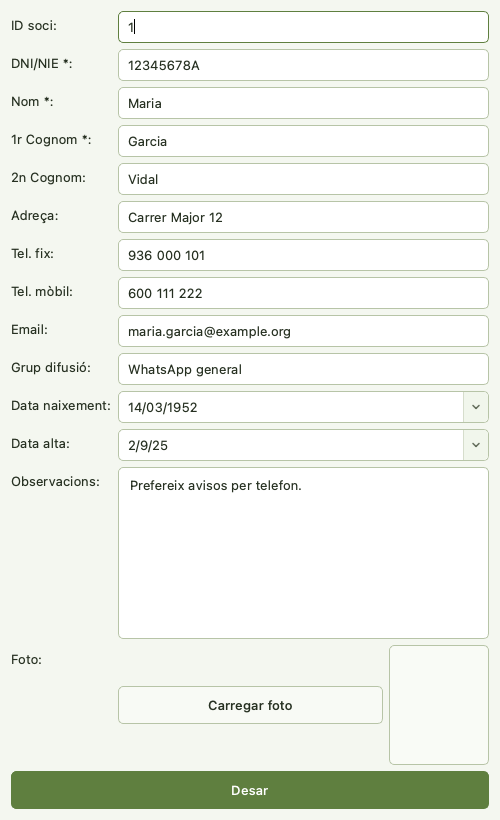
\includegraphics[width=0.52\textwidth]{./images/4_altaSocios.png}
  \caption{Formulario de alta o edición de socio.}
  \label{fig:nou-soci}
\end{figure}

Para crear un socio:
\begin{enumerate}
  \item Pulse \boton{Nou soci}.
  \item Rellene \campo{DNI/NIE}, \campo{Nom} y \campo{1r Cognom}. Son obligatorios.
  \item Si desea asignar un número de socio manual, rellene \campo{ID soci}. Si se deja vacío, se asigna automáticamente.
  \item Complete dirección, teléfonos, correo, grupo de difusión, fecha de nacimiento y observaciones.
  \item Pulse \boton{Carregar foto} si desea guardar una imagen del socio.
  \item Pulse \boton{Desar}.
\end{enumerate}

Campos principales:
\begin{longtable}{>{\bfseries}p{0.30\textwidth}p{0.62\textwidth}}
ID soci & Número interno del socio. Puede ser automático o manual.\\
DNI/NIE & Identificador único. No puede repetirse en otro socio.\\
Nom & Nombre del socio.\\
1r Cognom / 2n Cognom & Apellidos. El primer apellido es obligatorio en el formulario de alta.\\
Adreça & Dirección postal.\\
Tel. fix / Tel. mòbil & Teléfonos de contacto.\\
Email & Correo electrónico.\\
Grup difusió & Grupo o canal por el que se informa al socio.\\
Data naixement & Fecha de nacimiento. Puede dejarse vacía.\\
Data alta & Fecha de incorporación.\\
Observacions & Información interna relevante.\\
Foto & Imagen del socio para ficha o carnet.\\
\end{longtable}

\subsection{Editar socio desde el panel derecho}
\begin{enumerate}
  \item Seleccione el socio en la tabla.
  \item Modifique los campos en el panel derecho.
  \item Pulse \boton{Guardar}.
  \item Si desea abandonar cambios, pulse \boton{Descartar}.
\end{enumerate}

El panel derecho permite trabajar sin abrir el formulario completo. Es la opción más rápida para corregir teléfonos, correo, dirección, observaciones o fecha de baja.

\subsection{Baja de socio}
Para marcar la baja:
\begin{enumerate}
  \item Seleccione el socio.
  \item Active la casilla \campo{Baixa}.
  \item Introduzca la fecha de baja.
  \item Pulse \boton{Guardar}.
\end{enumerate}

La baja no equivale necesariamente a borrar el socio. Mantener el registro permite conservar historial de inscripciones, pagos y documentos.

\subsection{Eliminar socios}
La eliminación borra registros. Úsela solo cuando el socio se haya creado por error o cuando la entidad haya decidido retirar el registro.

Procedimiento general:
\begin{enumerate}
  \item Seleccione uno o varios socios en la tabla.
  \item Use la acción de eliminación disponible en la pestaña o el menú contextual.
  \item Revise el aviso.
  \item Confirme.
\end{enumerate}

Antes de eliminar socios con historial, haga una copia de seguridad.

\subsection{Exportar listado de socios}
Pulse \boton{Exportar PDF} para generar un listado de socios. El informe respeta los datos disponibles en la tabla y se abre con el visor PDF del sistema cuando es posible.

\subsection{Ficha, carnet y documentos}
Según las opciones visibles en la instalación, el socio seleccionado puede tener acciones para generar:
\begin{itemize}
  \item Carnet de socio.
  \item Ficha individual.
  \item Hoja imprimible de ficha y carnet.
  \item Documento LOPD.
\end{itemize}

Genere estos documentos después de comprobar que los datos personales y la fotografía son correctos.

\section{Inscripciones y pagos del socio}
\subsection{Abrir la ventana}
Para gestionar inscripciones de un socio, haga doble clic sobre su fila en la pestaña \menu{Socis}. Se abrirá \menu{Gestió d'inscripcions del soci}.

\begin{figure}[H]
  \centering
  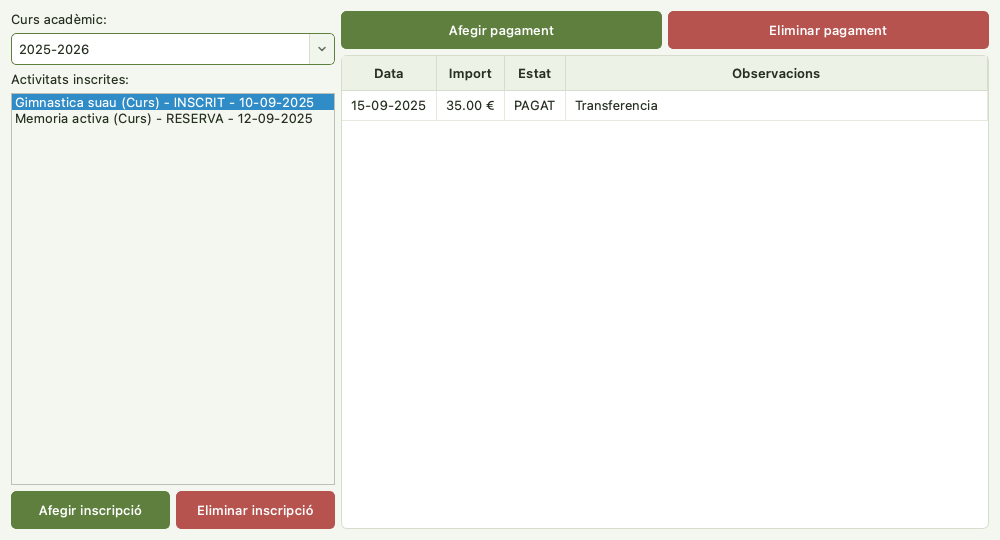
\includegraphics[width=\textwidth]{./images/5_pagament.png}
  \caption{Inscripciones de un socio y pagos asociados.}
  \label{fig:inscripciones}
\end{figure}

\subsection{Partes de la ventana}
\begin{itemize}
  \item \campo{Curs acadèmic}: filtra las inscripciones por curso o muestra todas.
  \item Lista \campo{Activitats inscrites}: muestra actividad, tipo, estado y fecha de inscripción.
  \item \boton{Afegir inscripció}: añade una actividad al socio.
  \item \boton{Eliminar inscripció}: borra la inscripción seleccionada.
  \item Tabla de pagos: muestra fecha, importe, estado y observaciones.
  \item \boton{Afegir pagament}: registra un pago en la inscripción seleccionada.
  \item \boton{Eliminar pagament}: elimina el pago seleccionado.
\end{itemize}

\subsection{Añadir una inscripción}
\begin{enumerate}
  \item Seleccione el curso académico.
  \item Pulse \boton{Afegir inscripció}.
  \item Elija la actividad disponible.
  \item Confirme.
\end{enumerate}

La aplicación evita duplicar la misma actividad para el mismo socio. Si la actividad tiene plazas disponibles, la inscripción se crea como \estado{INSCRIT}. Si no hay plazas, se crea como \estado{RESERVA}.

\subsection{Estados de inscripción}
\begin{itemize}
  \item \estado{INSCRIT}: el socio tiene plaza asignada.
  \item \estado{RESERVA}: el socio queda en lista de espera.
\end{itemize}

Cuando se elimina una inscripción con plaza, la aplicación puede actualizar reservas pendientes para cubrir la plaza libre.

\subsection{Eliminar una inscripción}
\begin{enumerate}
  \item Seleccione la inscripción en la lista izquierda.
  \item Pulse \boton{Eliminar inscripció}.
  \item Confirme el aviso.
\end{enumerate}

Revise antes si la inscripción tiene pagos. Si necesita conservar trazabilidad económica, valore anular el pago o dejar observaciones antes de borrar.

\subsection{Añadir un pago}
\begin{enumerate}
  \item Seleccione la inscripción.
  \item Pulse \boton{Afegir pagament}.
  \item Revise la fecha propuesta.
  \item Indique el importe. La ventana propone el precio de la actividad.
  \item Seleccione el estado \estado{PENDENT} o \estado{PAGAT}.
  \item Añada observaciones si procede.
  \item Pulse \boton{Afegir}.
\end{enumerate}

\subsection{Editar estado de pago}
La tabla de pagos permite editar determinados campos, especialmente el estado. Use esta opción para pasar un pago de pendiente a pagado cuando se confirme el ingreso.

\subsection{Eliminar un pago}
\begin{enumerate}
  \item Seleccione la inscripción.
  \item Seleccione el pago en la tabla derecha.
  \item Pulse \boton{Eliminar pagament}.
  \item Confirme.
\end{enumerate}

Use la eliminación solo para pagos creados por error. Para incidencias reales, documente la situación en observaciones.

\section{LOPD y firma digital}
\subsection{Objetivo}
La ventana \menu{Gesti\'o LOPD del soci} permite gestionar el documento de protección de datos de cada socio. Puede consultar documentos firmados, eliminarlos y preparar una firma digital desde tablet o móvil.

\begin{figure}[H]
  \centering
  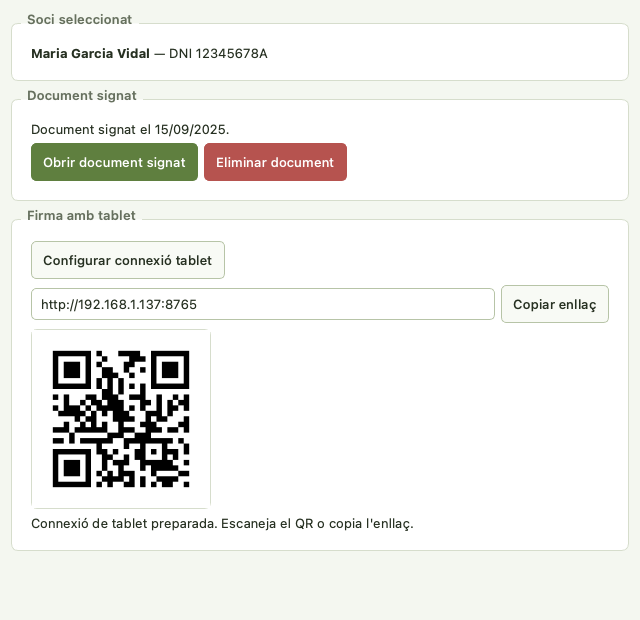
\includegraphics[width=0.72\textwidth]{./images/6_lopd.png}
  \caption{Gestión del documento LOPD y firma con tablet.}
  \label{fig:lopd}
\end{figure}

\subsection{Información visible}
La ventana muestra:
\begin{itemize}
  \item Datos básicos del socio seleccionado.
  \item Estado del documento firmado.
  \item Botones para abrir o eliminar el documento.
  \item Área de firma con tablet, enlace y código QR.
  \item Mensajes de progreso de la firma.
\end{itemize}

\subsection{Abrir documento firmado}
Si ya existe documento:
\begin{enumerate}
  \item Pulse \boton{Obrir document signat}.
  \item La aplicación abrirá el PDF con el visor del sistema.
  \item Revise que el documento corresponde al socio correcto.
\end{enumerate}

\subsection{Preparar firma con tablet}
\begin{enumerate}
  \item Abra la ventana LOPD del socio.
  \item Pulse \boton{Configurar connexió tablet}.
  \item La aplicación muestra un enlace y un código QR.
  \item Desde la tablet o móvil, conectados a la misma red, abra el enlace o escanee el QR.
  \item Complete la firma en el dispositivo.
  \item Espere a que la aplicación confirme que la firma se ha recibido y guardado.
\end{enumerate}

\subsection{Copiar enlace}
Pulse \boton{Copiar enllaç} para copiar la URL al portapapeles y enviarla o pegarla en el dispositivo de firma.

\subsection{Eliminar documento firmado}
\begin{enumerate}
  \item Pulse \boton{Eliminar document}.
  \item Confirme la eliminación.
  \item Revise que el estado vuelve a indicar que no hay documento firmado.
\end{enumerate}

Solo elimine el documento si se ha firmado por error, se ha asociado al socio incorrecto o existe un motivo administrativo claro.

\subsection{Problemas frecuentes de firma}
\begin{itemize}
  \item Tablet y ordenador no están en la misma red.
  \item El cortafuegos bloquea conexiones locales.
  \item La tablet pierde conexión antes de enviar la firma.
  \item Se ha abierto una URL antigua. Genere de nuevo el enlace.
\end{itemize}

\section{Actividades: cursos y viajes}
\subsection{Vista general}
La pestaña \menu{Activitats} permite gestionar tanto cursos como viajes. Dentro de ella hay dos subpestañas: \menu{Cursos} y \menu{Viatges}. El selector superior filtra por curso académico.

\begin{figure}[H]
  \centering
  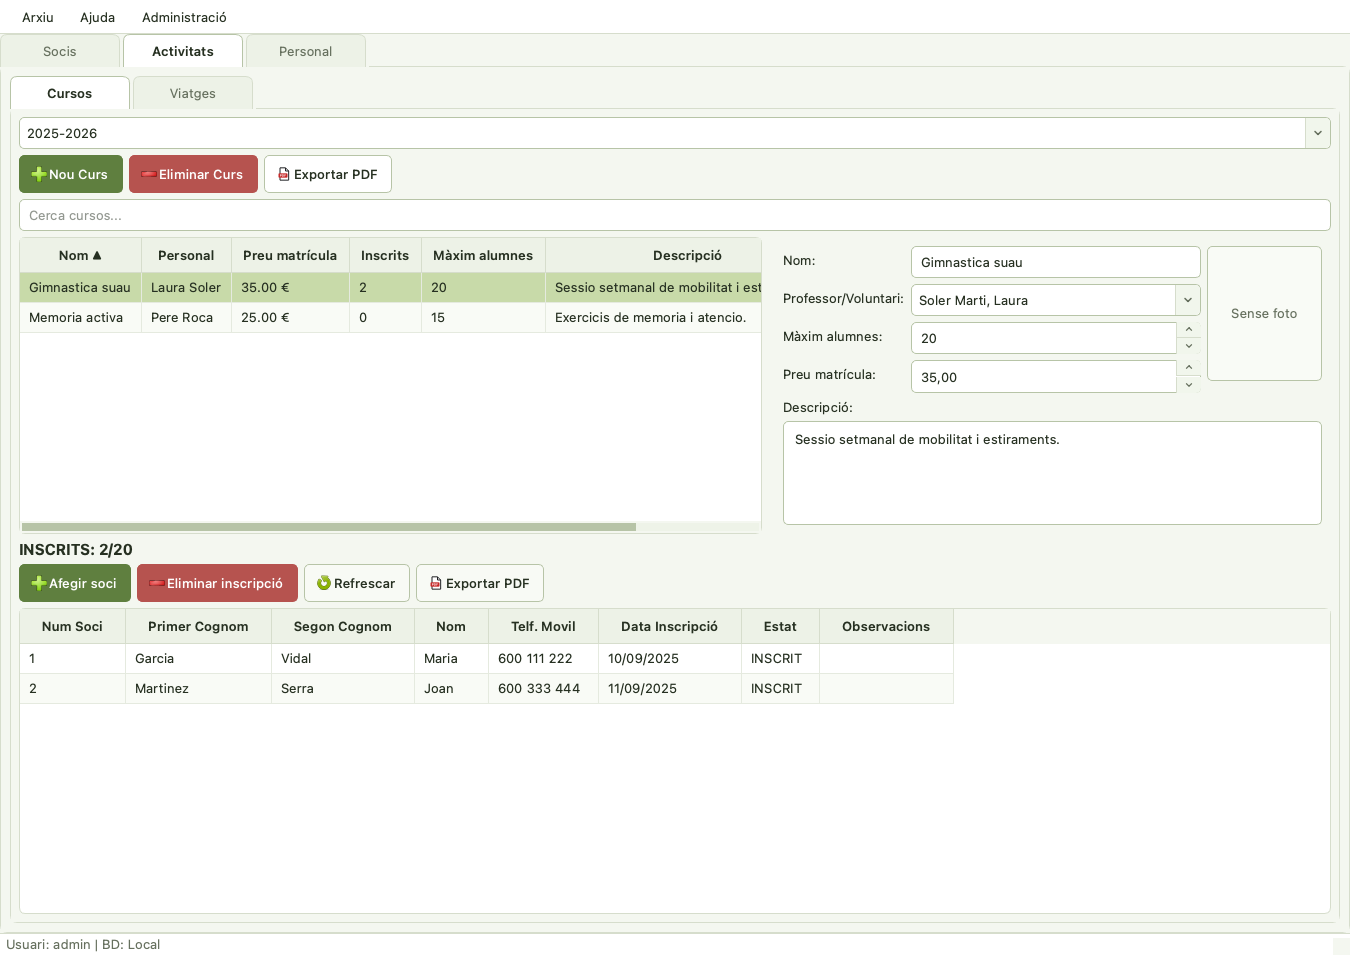
\includegraphics[width=\textwidth]{./images/7_activitats.png}
  \caption{Pestaña Activitats con listado, detalle e inscritos.}
  \label{fig:activitats}
\end{figure}

\subsection{Partes de la pestaña}
\begin{itemize}
  \item Selector de curso académico.
  \item Botones para crear, eliminar y exportar.
  \item Buscador de cursos o viajes.
  \item Tabla de actividades.
  \item Panel de detalle editable.
  \item Panel inferior de inscritos o participantes.
\end{itemize}

\subsection{Crear un curso o viaje}
\begin{figure}[H]
  \centering
  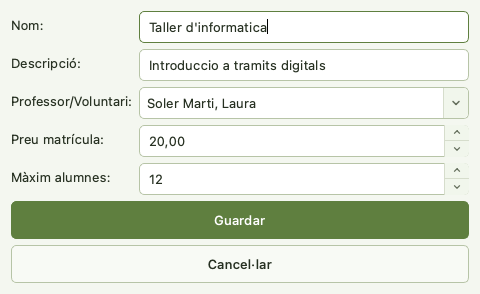
\includegraphics[width=0.58\textwidth]{./images/11_nou_curs.png}
  \caption{Formulario de creación de un nuevo curso.}
  \label{fig:nou-curs}
\end{figure}

Procedimiento:
\begin{enumerate}
  \item Seleccione el curso académico en el desplegable superior.
  \item Entre en \menu{Cursos} o \menu{Viatges}.
  \item Pulse \boton{Nou Curs} o \boton{Nou Viatge}.
  \item Rellene el nombre.
  \item Añada descripción o itinerario.
  \item Seleccione profesor, voluntario o responsable.
  \item Indique precio.
  \item Indique máximo de alumnos o plazas.
  \item Pulse \boton{Guardar}.
\end{enumerate}

Campos:
\begin{itemize}
  \item \campo{Nom}: nombre visible de la actividad.
  \item \campo{Descripció}: resumen del contenido o itinerario.
  \item \campo{Professor/Voluntari} o \campo{Responsable}: persona responsable.
  \item \campo{Preu matrícula} o \campo{Preu viatge}: importe de referencia para pagos.
  \item \campo{Màxim alumnes} o \campo{Places}: aforo máximo.
\end{itemize}

\subsection{Editar una actividad}
\begin{enumerate}
  \item Seleccione la actividad en la tabla.
  \item Modifique los campos del panel derecho.
  \item La aplicación guarda o refresca según el campo editado y el flujo de la pantalla.
  \item Revise que la tabla queda actualizada.
\end{enumerate}

Si cambia el precio, compruebe si afecta a pagos ya registrados. Los pagos existentes no deben modificarse automáticamente sin revisión.

\subsection{Eliminar una actividad}
\begin{enumerate}
  \item Seleccione la actividad.
  \item Pulse \boton{Eliminar Curs} o \boton{Eliminar Viatge}.
  \item Lea el mensaje, que incluye el nombre e identificador.
  \item Confirme solo si procede.
\end{enumerate}

Antes de eliminar actividades con inscritos, asistencia o pagos, haga una copia de seguridad.

\subsection{Gestionar inscritos desde Activitats}
El panel inferior muestra los inscritos de la actividad seleccionada. Desde ahí puede:
\begin{itemize}
  \item \boton{Afegir soci}: añadir un socio o participante.
  \item \boton{Eliminar inscripció}: quitar una inscripción.
  \item \boton{Refrescar}: actualizar el listado.
  \item \boton{Exportar PDF}: generar listado de inscritos.
\end{itemize}

\subsection{Participantes no socios}
Al añadir participantes desde la actividad, la aplicación puede permitir incorporar una persona no socia. En ese caso se registran nombre, apellidos, DNI, teléfono, correo y observaciones dentro de la inscripción, sin crear un socio completo.

\subsection{Cursos frente a viajes}
\begin{itemize}
  \item En \menu{Cursos}, los textos se orientan a profesores, matrícula, inscritos y máximo de alumnos.
  \item En \menu{Viatges}, los textos se orientan a responsable, precio del viaje, participantes y plazas.
\end{itemize}

\subsection{Exportar actividades}
Pulse \boton{Exportar PDF} para obtener un informe de las actividades visibles en el filtro actual. Compruebe el curso académico seleccionado antes de generar el documento.

\section{Asistencia}
\subsection{Abrir asistencia}
Desde la pestaña \menu{Activitats}, haga doble clic sobre un curso o use el menú contextual de la tabla para abrir \menu{Assistència}.

\begin{figure}[H]
  \centering
  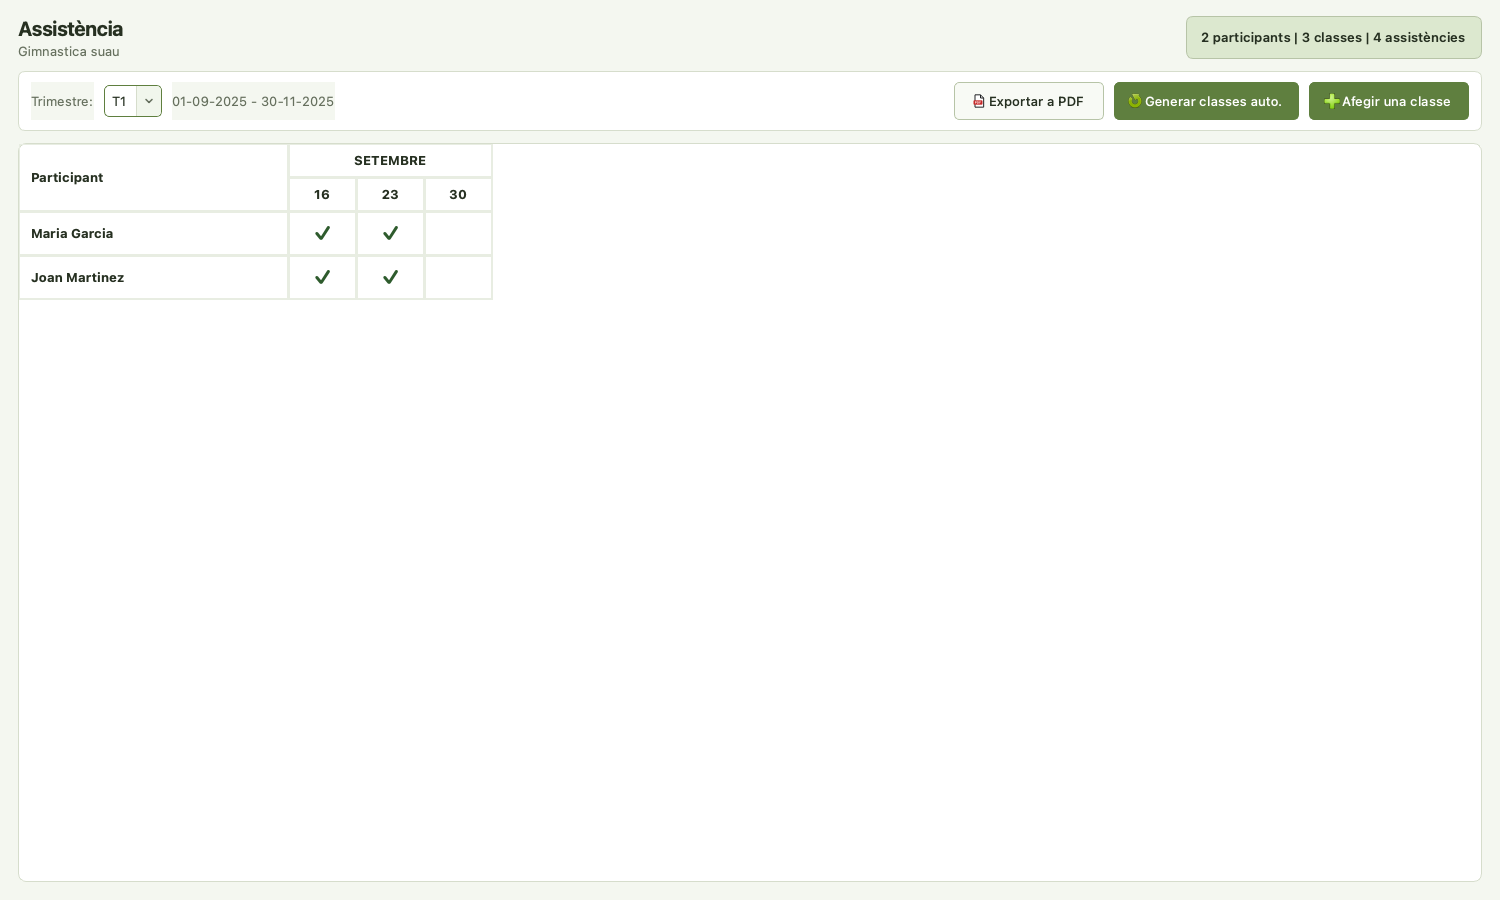
\includegraphics[width=\textwidth]{./images/8_asistencia.png}
  \caption{Control de asistencia de una actividad.}
  \label{fig:asistencia}
\end{figure}

\subsection{Partes de la ventana}
\begin{itemize}
  \item Título de la actividad.
  \item Selector de trimestre.
  \item Rango de fechas del trimestre.
  \item Resumen de participantes, clases y asistencias.
  \item Botones de exportación y creación de clases.
  \item Parrilla de asistencia.
\end{itemize}

\subsection{Seleccionar trimestre}
El desplegable \campo{Trimestre} filtra las clases y asistencias por trimestre. Si el trimestre no muestra fechas correctas, vuelva a la gestión de cursos académicos y revise la configuración.

\subsection{Generar clases automáticamente}
\begin{enumerate}
  \item Pulse \boton{Generar classes auto.}.
  \item Seleccione trimestre.
  \item Marque los días de la semana.
  \item Indique horario, duración y frecuencia si la ventana lo solicita.
  \item Confirme.
\end{enumerate}

Use esta opción para cursos recurrentes, por ejemplo sesiones semanales.

\subsection{Añadir una clase manual}
\begin{enumerate}
  \item Pulse \boton{Afegir una classe}.
  \item Seleccione trimestre y fecha.
  \item Indique hora o duración si corresponde.
  \item Guarde.
\end{enumerate}

Esta opción es útil para sesiones sueltas, recuperaciones o actividades especiales.

\subsection{Marcar asistencia}
La parrilla muestra participantes en filas y clases en columnas. Para marcar o desmarcar:
\begin{itemize}
  \item Pulse una celda para cambiar la asistencia individual.
  \item Revise que el símbolo aparece o desaparece correctamente.
  \item Compruebe el resumen superior si necesita confirmar totales.
\end{itemize}

\subsection{Eliminar clases}
La aplicación permite eliminar clases seleccionadas mediante la tecla \texttt{Supr} o acciones disponibles en la ventana. Confirme solo si la clase se creó por error. Al eliminar una clase también desaparecen sus asistencias.

\subsection{Exportar asistencia}
Pulse \boton{Exportar a PDF} para generar un informe de asistencia del trimestre o actividad. Revise el trimestre antes de exportar.

\section{Personal: profesores y voluntarios}
\subsection{Vista general}
La pestaña \menu{Personal} tiene dos subpestañas: \menu{Professors} y \menu{Voluntaris}. Ambas comparten una lógica similar: tabla, buscador, botones de alta/eliminación y panel de detalle.

\begin{figure}[H]
  \centering
  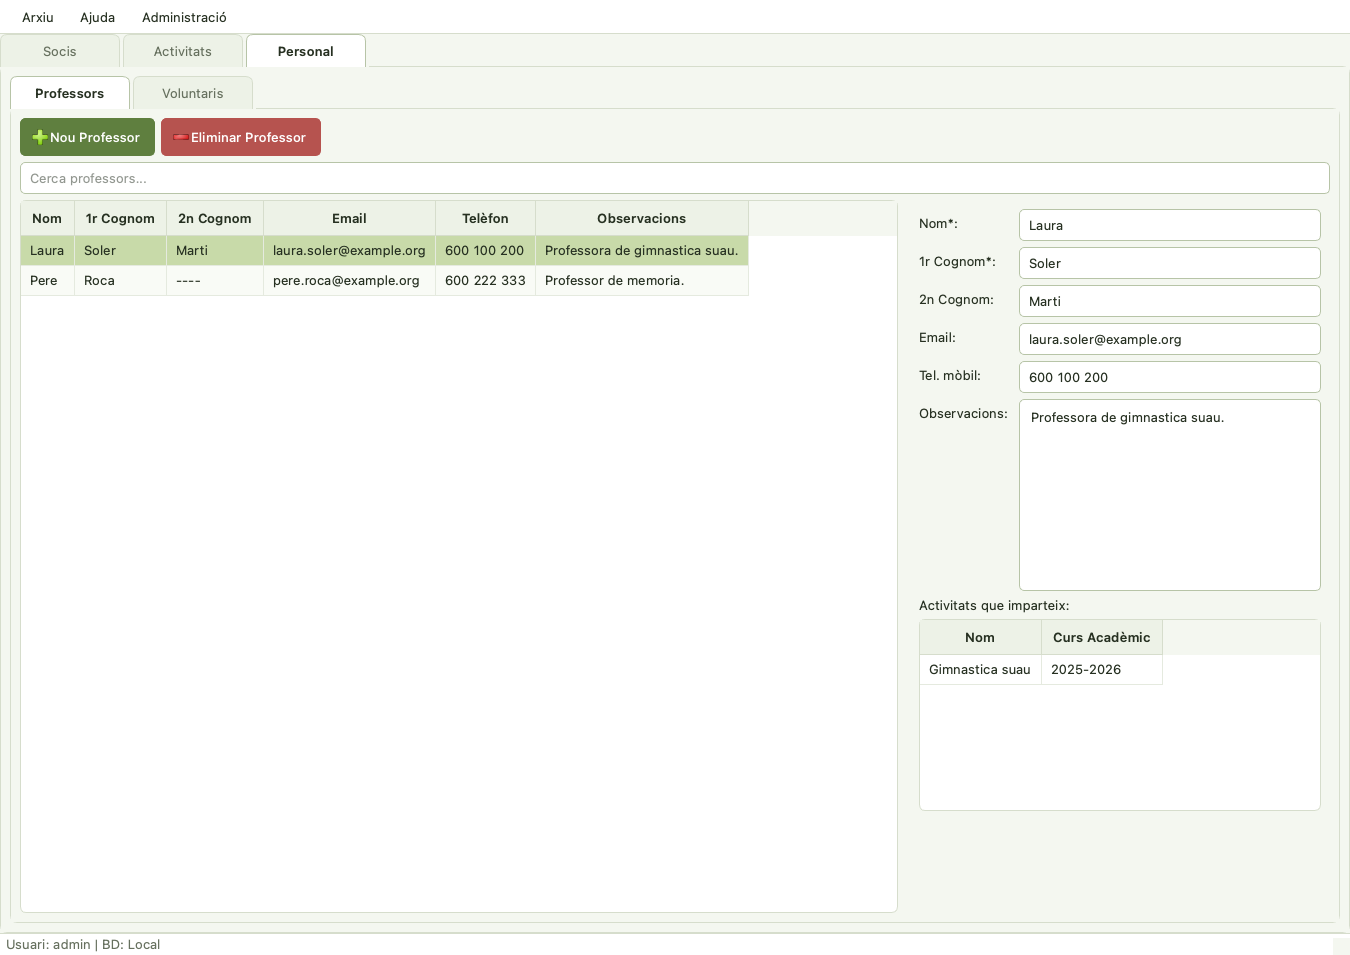
\includegraphics[width=\textwidth]{./images/9_personal.png}
  \caption{Gestión de profesores y voluntarios.}
  \label{fig:personal}
\end{figure}

\subsection{Alta de profesor}
\begin{enumerate}
  \item Abra \menu{Personal > Professors}.
  \item Pulse \boton{Nou Professor}.
  \item Rellene nombre, apellidos, correo, teléfono y observaciones.
  \item Guarde.
\end{enumerate}

\subsection{Alta de voluntario}
\begin{enumerate}
  \item Abra \menu{Personal > Voluntaris}.
  \item Pulse \boton{Nou Voluntari}.
  \item Rellene los datos.
  \item Guarde.
\end{enumerate}

\subsection{Editar personal}
\begin{enumerate}
  \item Seleccione una persona en la tabla.
  \item Modifique los campos del panel derecho.
  \item Guarde o espere al guardado según el comportamiento de la pantalla.
  \item Revise la tabla.
\end{enumerate}

\subsection{Actividades asociadas}
El panel de detalle muestra actividades que imparte o coordina la persona seleccionada. Esta información ayuda a evitar eliminar un profesor o voluntario que todavía aparece como responsable.

\subsection{Eliminar personal}
\begin{enumerate}
  \item Seleccione la persona.
  \item Pulse \boton{Eliminar Professor} o \boton{Eliminar Voluntari}.
  \item Revise el mensaje con nombre e identificador.
  \item Confirme.
\end{enumerate}

Antes de eliminar, compruebe si esa persona está asignada a actividades.

\section{Administración de usuarios}
\subsection{Acceso}
Solo los administradores pueden abrir \menu{Administració > Usuaris}.

\begin{figure}[H]
  \centering
  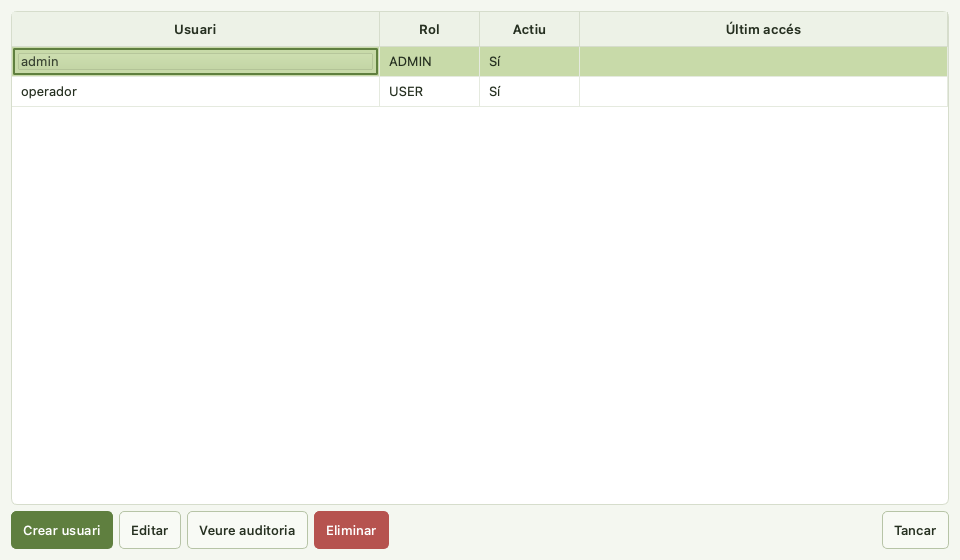
\includegraphics[width=0.92\textwidth]{./images/10_usuarios.png}
  \caption{Gestión de usuarios de la aplicación.}
  \label{fig:usuarios}
\end{figure}

\subsection{Tabla de usuarios}
La tabla muestra:
\begin{itemize}
  \item Usuario.
  \item Rol.
  \item Si está activo.
  \item Último acceso.
\end{itemize}

\subsection{Crear usuario}
\begin{enumerate}
  \item Pulse \boton{Crear usuari}.
  \item Introduzca el nombre de usuario.
  \item Introduzca y repita la contraseña.
  \item Seleccione rol \estado{USER} o \estado{ADMIN}.
  \item Active o desactive la casilla \campo{Actiu}.
  \item Pulse \boton{Desar}.
\end{enumerate}

\subsection{Roles}
\begin{itemize}
  \item \estado{USER}: acceso operativo normal.
  \item \estado{ADMIN}: acceso a usuarios, copias de seguridad y restauración local, además de las funciones normales.
\end{itemize}

Reserve \estado{ADMIN} para personal autorizado.

\subsection{Editar usuario}
\begin{enumerate}
  \item Seleccione un usuario.
  \item Pulse \boton{Editar}.
  \item Cambie rol, estado activo o contraseña.
  \item Si no desea cambiar la contraseña, deje los campos de contraseña vacíos.
  \item Pulse \boton{Desar}.
\end{enumerate}

\subsection{Desactivar frente a eliminar}
Para usuarios que ya no deben acceder, suele ser preferible desactivar la cuenta antes que eliminarla. Así se conserva la trazabilidad histórica de auditoría.

\subsection{Auditoría de usuario}
Pulse \boton{Veure auditoria} o haga doble clic sobre un usuario para consultar sus registros de auditoría. La ventana muestra fecha, acción, tabla, registro y detalle.

\subsection{Cambiar contraseña propia}
Cada usuario puede cambiar su contraseña desde \menu{Arxiu > Canviar contrasenya}. Debe introducir la contraseña actual y repetir la nueva.

\section{Importación de socios desde CSV o Excel}
\subsection{Formatos admitidos}
La aplicación acepta archivos:
\begin{itemize}
  \item \texttt{.xlsx}
  \item \texttt{.xls}
  \item \texttt{.csv}
\end{itemize}

\subsection{Proceso de importación}
\begin{enumerate}
  \item Abra \menu{Arxiu > Importar Socis (CSV/Excel)}.
  \item Seleccione el archivo.
  \item Espere a que avance la barra de progreso.
  \item Revise el resumen final.
  \item Si aparecen avisos, léalos en la ventana desplazable.
  \item Revise la pestaña \menu{Socis}, que se actualiza al terminar.
\end{enumerate}

\subsection{Avisos y errores}
La importación puede informar de:
\begin{itemize}
  \item Campos vacíos.
  \item DNI/NIE duplicados.
  \item Filas con formato incorrecto.
  \item Fechas no reconocibles.
  \item Registros que no se han podido crear.
\end{itemize}

Recomendación: haga una copia de seguridad antes de importaciones grandes.

\subsection{Buenas prácticas para preparar el archivo}
\begin{itemize}
  \item Revise que cada socio tenga DNI/NIE y nombre.
  \item Evite filas vacías en medio del listado.
  \item Use formatos de fecha consistentes.
  \item Elimine duplicados antes de importar.
  \item Guarde una copia del archivo original.
\end{itemize}

\section{Copias de seguridad y restauración}
\subsection{Crear copia de seguridad}
Disponible para administradores con base local SQLite.

\begin{enumerate}
  \item Abra \menu{Arxiu > Còpia de seguretat de la BD}.
  \item Elija la carpeta de destino.
  \item Mantenga el nombre sugerido o escriba otro nombre.
  \item Guarde.
  \item Espere el mensaje \menu{Còpia creada}.
\end{enumerate}

El nombre sugerido incluye fecha y hora. Guarde las copias en una ubicación segura.

\subsection{Restaurar una copia}
\begin{enumerate}
  \item Abra \menu{Arxiu > Restaurar BD des d'una còpia}.
  \item Lea el aviso: la base actual se sobrescribirá.
  \item Confirme.
  \item Seleccione el archivo \texttt{.db}.
  \item Espere a que la aplicación restaure la base.
\end{enumerate}

Advertencia: restaurar sustituye los datos actuales por los del archivo seleccionado. Antes de restaurar, cree una copia de la base actual.

\subsection{Bases externas PostgreSQL}
La copia y restauración integradas solo están disponibles para SQLite. Si trabaja con PostgreSQL, use herramientas del servidor como \texttt{pg\_dump}, \texttt{pg\_restore}, \texttt{psql} o las copias gestionadas del proveedor.

\section{Actualizaciones}
\subsection{Comprobación automática}
La aplicación empaquetada puede comprobar si existe una versión más reciente. Si hay una actualización, se muestra una ventana con:
\begin{itemize}
  \item Versión actual.
  \item Nueva versión.
  \item Resumen de la release, si existe.
  \item Botones para instalar, posponer o ver la release.
\end{itemize}

\subsection{Comprobación manual}
Abra \menu{Ajuda > Comprovar actualitzacions manualment}. En modo desarrollo, la aplicación informa de que esta función solo está disponible en la versión empaquetada.

\subsection{Instalar actualización}
Antes de instalar:
\begin{enumerate}
  \item Guarde cambios pendientes.
  \item Cierre trabajos abiertos.
  \item Haga una copia de seguridad si se han introducido datos importantes.
  \item Pulse \boton{Instal·lar ara}.
\end{enumerate}

Durante la instalación aparece una ventana de progreso. Al terminar, la aplicación se cierra para completar el proceso.

\section{Informes y PDFs}
\subsection{Dónde se generan informes}
La aplicación genera PDF desde diferentes puntos:
\begin{itemize}
  \item \boton{Exportar PDF} en \menu{Socis}: listado de socios.
  \item \boton{Exportar PDF} en \menu{Activitats}: listado de cursos o viajes.
  \item \boton{Exportar PDF} en inscritos: listado de participantes.
  \item \boton{Exportar a PDF} en asistencia: informe de asistencia.
  \item Acciones de carnet, ficha o LOPD: documentos individuales del socio.
\end{itemize}

\subsection{Recomendaciones para archivar PDFs}
\begin{itemize}
  \item Use nombres descriptivos con curso, actividad y fecha.
  \item Guarde los documentos en carpetas compartidas con acceso restringido.
  \item No almacene documentos LOPD en ubicaciones públicas.
  \item Revise el PDF antes de imprimir o enviar.
\end{itemize}

\section{Flujos de trabajo completos}
\subsection{Alta completa de un nuevo socio}
\begin{enumerate}
  \item Abra \menu{Socis}.
  \item Pulse \boton{Nou soci}.
  \item Introduzca DNI/NIE, nombre y apellidos.
  \item Complete teléfonos y correo.
  \item Añada grupo de difusión y observaciones.
  \item Cargue foto si está disponible.
  \item Guarde.
  \item Seleccione el socio en la tabla.
  \item Abra LOPD y gestione la firma.
  \item Haga doble clic en el socio para inscribirlo en actividades.
\end{enumerate}

\subsection{Crear curso anual y actividades}
\begin{enumerate}
  \item Cree el curso académico.
  \item Revise trimestres.
  \item Cree profesores y voluntarios.
  \item Abra \menu{Activitats}.
  \item Seleccione el curso académico.
  \item Cree cursos y viajes.
  \item Revise aforo y precio.
  \item Exporte el listado si necesita revisión interna.
\end{enumerate}

\subsection{Inscribir y cobrar una matrícula}
\begin{enumerate}
  \item Busque al socio.
  \item Haga doble clic.
  \item Seleccione el curso académico.
  \item Pulse \boton{Afegir inscripció}.
  \item Elija actividad.
  \item Seleccione la inscripción creada.
  \item Pulse \boton{Afegir pagament}.
  \item Revise importe.
  \item Marque \estado{PAGAT} si ya se ha cobrado o \estado{PENDENT} si queda pendiente.
  \item Guarde el pago.
\end{enumerate}

\subsection{Preparar asistencia de un curso}
\begin{enumerate}
  \item Abra \menu{Activitats}.
  \item Seleccione el curso académico y la actividad.
  \item Revise que haya inscritos.
  \item Abra asistencia con doble clic.
  \item Seleccione trimestre.
  \item Genere clases automáticamente o añádalas una a una.
  \item Marque asistencia tras cada sesión.
  \item Exporte PDF al final del trimestre.
\end{enumerate}

\subsection{Cierre de trimestre}
\begin{enumerate}
  \item Revise asistencia de cada actividad.
  \item Exporte informes de asistencia.
  \item Revise pagos pendientes.
  \item Exporte listados de inscritos si se requieren.
  \item Haga copia de seguridad.
\end{enumerate}

\section{Buenas prácticas generales}
\begin{itemize}
  \item Cree copias de seguridad antes de importaciones, restauraciones o borrados importantes.
  \item Use cuentas personales, no compartidas.
  \item Mantenga actualizados teléfonos y correos.
  \item No reutilice DNI/NIE ficticios para socios reales.
  \item Compruebe el curso académico seleccionado antes de crear actividades o informes.
  \item Evite eliminar registros con historial si puede marcarlos como baja o inactivos.
  \item Documente incidencias en observaciones.
  \item Revise las reservas después de bajas o eliminaciones de inscripción.
  \item Controle quién tiene rol \estado{ADMIN}.
  \item Archive PDFs sensibles con permisos adecuados.
\end{itemize}

\section{Resolución de problemas}
\subsection{No puedo entrar}
\begin{itemize}
  \item Revise usuario y contraseña.
  \item Compruebe el perfil de conexión.
  \item Si usa base externa, confirme conexión a internet o red interna.
  \item Pida a un administrador que revise si su usuario está activo.
\end{itemize}

\subsection{No aparece una actividad}
\begin{itemize}
  \item Compruebe el curso académico seleccionado.
  \item Revise si está en \menu{Cursos} o \menu{Viatges}.
  \item Borre el texto del buscador.
  \item Verifique que la actividad no se eliminó.
\end{itemize}

\subsection{No puedo crear una actividad}
\begin{itemize}
  \item Debe existir un curso académico.
  \item Debe seleccionarse un curso concreto, no solo \menu{Tots els cursos}.
  \item El nombre de la actividad es obligatorio.
  \item Revise que exista personal si desea asignar responsable.
\end{itemize}

\subsection{Un socio no se guarda}
\begin{itemize}
  \item Revise campos obligatorios.
  \item Compruebe si el DNI/NIE ya existe.
  \item Si asigna ID manual, confirme que no está usado.
  \item Revise que las fechas sean válidas.
\end{itemize}

\subsection{La importación falla}
\begin{itemize}
  \item Verifique el formato del archivo.
  \item Cierre el Excel antes de importar.
  \item Revise columnas obligatorias.
  \item Corrija errores mostrados en la ventana de avisos.
  \item Pruebe primero con una muestra pequeña.
\end{itemize}

\subsection{No se genera un PDF}
\begin{itemize}
  \item Compruebe que hay datos para exportar.
  \item Verifique permisos de la carpeta de destino.
  \item Cierre el PDF si ya está abierto en otro programa.
  \item Revise mensajes de error.
\end{itemize}

\subsection{La firma LOPD no conecta}
\begin{itemize}
  \item Tablet y ordenador deben estar en la misma red.
  \item Vuelva a generar el enlace.
  \item Use el QR visible en pantalla.
  \item Compruebe si el cortafuegos bloquea conexiones locales.
\end{itemize}

\subsection{La asistencia no muestra alumnos}
\begin{itemize}
  \item Revise que la actividad tenga inscritos.
  \item Compruebe el curso académico.
  \item Seleccione el trimestre correcto.
  \item Refresque la actividad si acaba de cambiar inscripciones.
\end{itemize}

\section{Glosario}
\begin{longtable}{>{\bfseries}p{0.28\textwidth}p{0.64\textwidth}}
Soci & Persona asociada a la entidad.\\
Curs Academic & Periodo anual de gestión.\\
Trimestre & Subperiodo dentro del curso académico.\\
Activitat & Curso o viaje.\\
Inscripció & Registro que une un socio con una actividad.\\
INSCRIT & Estado de inscripción con plaza asignada.\\
RESERVA & Estado de inscripción en lista de espera.\\
Pagament & Pago asociado a una inscripción.\\
PENDENT & Pago pendiente de confirmar o cobrar.\\
PAGAT & Pago realizado.\\
LOPD & Documento de protección de datos del socio.\\
Professor & Persona que imparte cursos.\\
Voluntari & Persona que colabora o coordina actividades.\\
ADMIN & Usuario con permisos administrativos.\\
USER & Usuario operativo normal.\\
\end{longtable}

\end{document}
